\section{A Unified Language}
\label{lang}

\newcommand\semp[1]{[\![{#1}]\!]}
\newcommand\fix{\operatorname{fix}}

For the purpose of manipulating programs and reasoning about them,
we first set up a small language that can easily express our programs (that is,
partially transformed specifications), and can also be translated to executable
code in a straightforward fashion. We choose a functional
setting, with scalar types for array indices ($i, j, k : J$ in the example)
and values stored in the arrays, typically real numbers ($G_{ij} : \R$ in the example).
Arrays are encoded as functions, or arrow types, mapping indices
to values (e.g. $G : J^2\to\R$). We want to have a notion of
array elements that are uninitialized, so we assume every scalar type
contains the special value $\bot$, corresponding to an undefined value.

Our language should be able to express operations such as \textsf{Slice}
from the previous section. To achieve this, we introduce 
\newterm{predicate abstraction} over the index types, by extending the
type system with subtyping and \newterm{refinement types}. An index
type $J$ can be partitioned into subtypes $\langle J_0 \,|\, J_1\rangle$
(two or more), meaning that we define predicates $\widehat{J}_0,\widehat{J}_1 : J\to\B$ (where $\B$ is the Boolean type)
and the refinement types $J_0=\{v\,{:}\,J \,|\, \widehat{J}_0(v)\}$
and $J_1=\{v\,{:}\,J \,|\, \widehat{J}_1(v)\}$, which become subtypes of $J$.
Usually, we can omit the ``hat'' and use $J_0$ as a synonym for $\widehat{J}_0$ 
when it is clear from the context that it designates a type. 
We would then provide types for sub-arrays, e.g. 
$G^{\raisebox{-2pt}{\tinyqbox{2}}} : J_0\times J_1 \to \R$.

To refer to a region of a given array, we define a \newterm{guard}
operator, which is parameterized by subtypes of the indices,
for example $G^{\raisebox{-2pt}{\tinyqbox{2}}} = [G]_{J_0\times J_1}$.
To combine computations on different parts of the array, we use a lifting
of the ternary condition operator (known as {\tt ?:}) to functions,
where the condition is implied by the operands; e.g.
(\Cref{overview:quadrants})
\[
G=G^{\tinyqbox1} \big/ G^{\tinyqbox2} \big/ G^{\tinyqbox4} = 
\lambda ij.
\begin{cases}
  G^{\tinyqbox1}_{ij} & i,j\in J_0 \\
  G^{\tinyqbox2}_{ij} & i\in J_0 \land j\in J_1 \\
  G^{\tinyqbox4}_{ij} & i,j\in J_1 \\
\end{cases}
\]

\bigskip
\begin{paragraph}{Formal set-up}The Bellmania language is based on the polymorphic
$\lambda$-calculus, that is, simply typed $\lambda$-calculus with universally quantified type variables 
(also known as \newterm{System F}).
The following subsections contain formal definitions for language constructs.
\end{paragraph}

We write abstraction terms as $(v:\T)\mapsto e$, where $\T$ is the type of the argument $v$ and $e$ is
the body, instead of the traditional notation $\lambda(v:\T).\,e$, mainly due to aesthetic reasons
but also because we hope this will look more familiar to intended users.
Curried functions $(v_1\,{:}\,\T_1)\mapsto (v_2\,{:}\,\T_2) \mapsto \cdots \mapsto (v_n\,{:}\,\T_n) \mapsto e$ are abbreviated 
as $(v_1\,{:}\,\T_1)\cdots(v_n\,{:}\,\T_n)\mapsto e$. Argument types may be omitted when
they can be inferred from the body.

The semantics differ slightly from that of traditional functional languages: arrow types $\T_1\to\T_2$
are interpreted as {\bf mappings} from values of type $\T_1$ to values of type $\T_2$. Algebraically,
interpretations of types, $\semp{\T_1}$, $\semp{\T_2}$, are sets, and interpretations of arrow-typed terms,
$f : \T_1\to\T_2$, are {\bf partial functions} --- $\semp{f} : \semp{\T_1}\rightharpoonup\semp{\T_2}$.
This implies that a term $t : \T$ may have an \newterm{undefined} value, $\semp{t}=\bot_\T$
(We would shorten it to $\semp{t}=\bot$ when the type is either insignificant or understood from the context).
For simplicity, we shall identify $\bot_{\T_1\to\T_2}$ with the empty mapping $(v:\T_1)\mapsto\bot_{\T_2}$.

All functions are naturally extended, so that $f\,\bot=\bot$.

\subsection{Operators}
\label{lang:operators}

The core language is augmented with the following intrinsic operators:

\begin{itemize}
  \item A fixed point operator $\fix f$, with denotational semantics
    \[\semp{\fix f} ~=~ \theta \textrm{ ~ s.t. ~ } \semp f\,\theta=\theta\]
  we assume that recurrences given in specifications are well-defined, 
  such that $\semp f$ has a single fixed point.
  In other words, we ignore nonterminating computations ---
  we assume that the user provides only terminating recurrences in specifications.%\rsc{This sounds like we have a way of figuring out if a computation is non-terminating. Do we? Can we get rid of this last statement?}
  \item A guard operator $[\,]_{_\square}\,$, which comes in two flavors: 
  \[\begin{array}{l}
      [x]_{\mathit{cond}} = \begin{cases}x & \mathit{cond} \\ \bot & \lnot\mathit{cond}\end{cases} \\
      {}[f]_{P_1\times P_2\times \cdots P_n} = \overline{x} \mapsto [f\,\overline{x}]_{\bigwedge P_i(x_i)} 
    \end{array}\]
  where $\overline{x} = x_1 \cdots x_n$. This second form can be used to
  refer to quadrants of an array; in this form, it always produces a term of
  type $\square\to\mathcal{R}$, where $\mathcal{R}$ is the domain of $f$.
  \item A slash operator $/$~:     \vspace{-2pt}
  \[\renewcommand\arraystretch{1.5}
    \begin{array}{ll}
      \mbox{For scalars $x,y:\S$} & x/y = \begin{cases}x & \mbox{if }x\neq\bot \\ y & \mbox{if }x=\bot\end{cases} \\
      \mbox{For $f,g:\T_1\to\T_2$} & f/g = (v:\T_1)\mapsto (f\,v)/(g\,v)
    \end{array}\]
  This operator is typically used to combine computations done on
  parts of the array. For example, \[\psi\mapsto \big[f\,\psi\big]_{I_0} ~ \Big/ ~ \big[g\,\psi\big]_{I_1}\]
  combines a result of $f$ in the lower indices of a (one-dimensional) array
  with a result of $g$ in the higher indices ($I_0$ and $I_1$, respectively, are the index subsets).
  Notice that this does not limit the areas from which $f$ and $g$ read;
  they are free to access the entire domain of $\psi$.
\end{itemize}

In our concrete syntax, function application and $\fix$ take precedence over $/$,
and the body of $\mapsto$ spans as far as possible (like $\lambda v$ in $\lambda$-calculus).

\subsection{Primitives}

The standard library contains some common primitives:

\newcommand\forallT{\forall\T\!.~}
\newcommand\forallTS{\forall\T\S\!.~}


\begin{itemize}
  \item $\R$, a type for real numbers; $\N$ for natural numbers; $\B$ for Boolean true/false.
  \item ${=} : \forallT \T\to\T\to\B$, always interpreted as equality.
  \item ${+}, {-} : \forallT \T\to\T\to\T$, polymorphic binary operators.
  \item ${<} : \forallT \T\to\T\to\B$, a polymorphic order relation.
  \item $cons : \forallT \T\to(\N{\to}\T)\to(\N{\to}\T), nil : \forallT \N\to\T$, list constructors.
  \item $\min, \max, \Sigma : \forallTS (\T\to\S)\to\S$, reduction (aggregation) operators
    on ordered/unordered collections. The collection is represented by a mapping $f : \T\to\S$,
    so that e.g. \[\semp{\min f} = \min \big\{\semp{f}\,v \;\big|\; v\in\semp{\T}, \semp{f}\,v\neq\bot\big\}\]
    The collections are assumed to be finite.
\end{itemize}

\subsection{Additional Notation}

We also adopt some syntactic sugar to make complex terms more manageable:

\begin{itemize}
  \item $x \applt f ~=~ f\,x$ for application from the left.
  \item $\langle t_1,\cdots,t_n\rangle = cons~t_1 ~ (cons \cdots (cons~t_n ~ nil) \cdots)$
    for fixed-length lists.
\end{itemize}

\subsection{Types and Type Qualifiers}
\label{lang:types}

We extend the type system with predicate abstraction in the form of logically qualified data types 
(Liquid Types~\cite{PLDI08/Rondon}). 
These are refinement types that provide a natural encoding of predicate abstraction
by restricting refinements to set of abstraction predicates,
called \newterm{qualifiers}, which are defined over the base types.
Contrary to their general use, the purpose of these qualifiers in Bellmania is not to
check a program for safety and reject ill-typed programs, but rather to serve as annotations for
tactics, to convey information to the solver for use in proofs, and later to help the compiler
properly emit memory access and parallelization primitives.

More specifically, typing $f : \{v:\T_1 ~|~ P(v)\}\to\T_2$ would mean that $f\,x$
can only be defined where $P(x)$ is true; otherwise, $f\,x=\bot$. 
It {\bf does not} mean that the compiler has to prove $P(x)$ at the point where the term $f\,x$
occurs.

As such, we define a Bellmania program to be well-typed iff it is well-typed
without the annotations (in its \newterm{raw form}). Qualifiers are processed
as a separate pass to properly annotate sub-terms.

Some qualifiers are built-in, and more can defined by the user. To keep the syntax simple, we somewhat
limit the use of qualifiers, allowing only the following forms:

\begin{itemize}
  \item $\{v:\T ~|~ P(v)\}$, abbreviated as $\T\cap P$. When the signature of $P$ is known (which is
  usually the case), it is enough to write the type as $P$.
  \item $\{v:\T ~|~ P(v)\land Q(v)\}$, abbreviated as $\T\cap P\cap Q$, or just $P\cap Q$. This extends
  to any number of conjuncts of the same form.
  \item $(x : \T_1) \to \{v:\T_2 ~|~ R(x,v)\} \to \T_3$, abbreviated as $\big((\T_1\times\T_2)\cap R\big)\to\T_3$.
  The qualifier argument $x$ {\bf must} be the preceding argument; this extends to predicates of
  any arity (that is, a $k$-ary predicate in a qualifier is applied to the $k$
  arguments to the left of it, including the one where it appears).
\end{itemize}


\medskip  
The type refinement constructors $\cap$ and $\times$ may be composed to create \newterm{droplets} (tiny bits of liquid),
using the abstract syntax in \Cref{lang:droplets}.
Note that the language does not include tuple types; hence all function types are
implicitly curried, even when using $\times$.
Droplets can express conjunctions of qualifiers,
as long as their argument sets are either disjoint or contained, but not overlapping;
for example, \[x:\{v:\T_1~|~P(v)\}\to \{v:\T_2~|~Q(v)\land R(x,v)\}\to\T_3\] can be written as
$\big((P\times Q)\cap R\big)\to\T_3$, but \[x:\T_1\to y:\{v:\T_2~|~R(x,v)\} \to \{v:\T_3~|~R(y,v)\}\to\T_4\]
cannot be represented as a droplet, except by extending the vocabulary of qualifiers.

\cbstart\diffnote{motivate droplets}%
Through the use of droplets, we manage to harness refinement types without being to 
cumbersome and requiring the user to write verbose annotations.
To this end, we trade off some expressive power for succinctness.
\cbend

\exampleTitle

\noindent
The specification of the Parenthesis problem (\Cref{overview:paren spec}) will be written as

\vspace{-5mm}
\newcommand\Jsquaredlt{J^2\!\!\!{\scriptscriptstyle _{<}}}
\[
  \renewcommand\arraystretch{1.2}
  \begin{array}{@{}l@{}l@{}l@{}}
    \lspan2{x : J \to \R} \\
    \lspan2{w : J^3 \to \R} \\
    G ~=~ \fix~(\theta:\Jsquaredlt\to\R)\,i\,j \mapsto{}
      & \big[x_i\big]_{i+1=j} ~\Big/ \\
      & \min k\mapsto\theta_{ik}+\theta_{kj}+w_{ikj}
  \end{array}
\]

$\Jsquaredlt$ is used here as an abbreviation for $(J{\times}J)\,{\cap}\,{<}$.
We also use $f_{xy}$
as a more readable typographic alternative for $f\,x\,y$,
where $f$ is a function and $x$, $y$ are its arguments.

Note that the range for $k$ in $\min k\mapsto\cdots$ is implicit, given the type of
$\theta$: 
\vspace{-.5em}
\[\theta_{ik}\neq\bot\implies i<k \quad \mbox{and} \quad \theta_{kj}\neq\bot\implies k<j\]

\vspace{-.5em}
\hrule
\medskip

\iffalse
\newcommand\examplePar{%
\vspace{1pt}\noindent\hspace{-2pt}%
\tikz[baseline=(E.base)]\node(E)[rectangle,draw=black!40!white,rounded corners=.7em] {\bf Example.};
}
\examplePar
The array $G$ computed in the Parenthesis example (\Cref{overview:paren spec}) can be typed using:
\[
\begin{array}{l}
  G : ((J\times J)\cap{<}) \to \R \\
\end{array}
\]

This states that $G\,i\,j$ is only defined for $i<j$. It doesn't {\em force} it to be defined,
as it is still a partial function.
\fi

\subsubsection*{Typing Rules}

\begin{figure}
\[
\begin{array}{lcll}
  d       & ::= & e^1 \quad |\quad e^k\to d \\
  e^1     & ::= & \T & \mbox{\it\small for scalar type $\T$} \\
  e^{k+l} & ::= & e^k \times e^l \\
  e^k     & ::= & e^k \cap P & \mbox{\it\small for $k$-ary predicate symbol $P$} 
\end{array}
\]
\vspace{-.5em}
\caption{\label{lang:droplets}
  Syntax of type qualifiers (droplets). $k$, $l$ are positive integers
  that stand for dimension indexes.}
\end{figure}

As mentioned earlier, annotations are ignored when typechecking a term.
This gives a simple characterization of type safety without the need to
explictly write any new typing rules. It also means that for $f:\T_1\to\T_2$, $x:\T_3$, we obtain $f\,x:\T_2$ whenever
$\T_1$ and $\T_3$ have the same \newterm{shape} (the raw type obtained by removing all qualifiers).
This requires some explanation.

Considering a (partial) function $\T\to\S$ to be a set of pairs of elements $\langle x,y\rangle$ 
from its domain $\T$ and range $\S$, respectively, it is clear to see that any function of type $\T_1\to\S_1$,
such that $\semp{\T_1}\subseteq\semp{\T}$, $\semp{\S_1}\subseteq\semp{\S}$, 
is \emph{also}, by definition, a function of type $\T\to\S$, since $\semp{\T_1}\times\semp{\S_1}\subseteq\semp{\T}\times\semp{\S}$.
If we define subtyping as inclusion of the domains, i.e. $\T_1 <:\T$ whenever $\semp{\T_1}\subseteq\semp{\T}$,
this translates into:
%
\[\T_1<:\T ~\land~ \S_1<:\S ~~\Rightarrow~~ (\T_1\to\S_1) <: (\T\to\S)\]

In this case, the type constructor $\to$ is {\bf covariant} in both arguments.\footnote{This is different from classical view, and holds in this case because we chose to interpret functions as \emph{mappings} (see beginning of this section).}
With this in mind, a function $g:(\T\to\S)\to \S_2$ can be called with an argument $a: \T_1\to\S_1$,
by regular subtyping rules, and $g\,a : \S_2$.

When the argument's type is not a subtype of the expected type, but has the same shape,
it is \newterm{coerced} to the required type by restricting values to the desired proper subset.
%
\[\mbox{For }h:\T\to\S \qquad \semp{h\,a} ~=~ \semp{h}\big(\semp{a} :: \T\big)\]

Where $::$ is defined as follows:
\begin{itemize}
  \item For scalar (non-arrow) type $\T$, \[x :: \T ~=~ \begin{cases}x & \mbox{if }x\in\semp{\T} \\ \bot & \mbox{if }x\not\in\semp{\T}\end{cases}\]
  \item $f :: \T\to\S ~=~ x\mapsto \big(f\,(x :: \T)\big) :: \S$
\end{itemize}

\medskip
We extend our abstract syntax with an explicit \newterm{cast operator}
$t::\T$ following this semantics. Notice that this is not the same as $t:\T$, which is a \emph{type judgement}.

\subsubsection*{Type Inference}

\begin{figure*}
\vspace{-8mm}
\newcommand\typerule[2]{{\renewcommand\arraystretch{1.5}\begin{array}[t]{c} #1 \\ \hline #2 \end{array}}}
\[
\renewcommand\arraystretch{2.8}
\begin{array}{cccp{1cm}}
  \multirow{2}{1cm}[-2em]{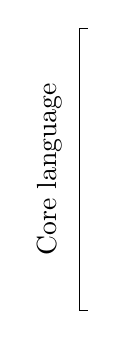
\begin{tikzpicture}\draw (0,0) -- ++(-1mm,0) -- ++(0,-10.2em) {} node[midway,anchor=base,xshift=-3mm,rotate=90] {Core language} -- ++(1mm,0);\end{tikzpicture}} &
  \typerule{e=v \qquad \Gamma,v:\T_1\vdash e:\T_0}
           {\Gamma,v:\T_1 ~\vdash~ e:\T_0\sqcap\T_1} &
  \typerule{e=e_1\,e_2 \qquad \Gamma \vdash e:\T, ~ e_1:\T_1\to\S_1, ~ e_2:\T_2}
           {\renewcommand\arraystretch{1.2}
            \begin{array}[t]{@{}l@{}l@{}}
              \Gamma ~\vdash~ & e:\T\sqcap\S_1,  \quad
                                e_2:\T_1\sqcap\T_2, \\
                              & e_1:(\T_1\to\S_1)\sqcap(\T_2\to\T)
            \end{array}} & \\
  &
  \cspan2{
  \typerule{e=(v:\T)\mapsto e_1 \qquad \Gamma\vdash e:\T_0\to\S_0 \qquad \Gamma,v:\T\sqcap\T_0\vdash e_1:\T_1}
           {\renewcommand\arraystretch{1.2}
            \begin{array}[t]{r@{}l}
              \Gamma ~\vdash~ & e:(\T_0\to\S_0)\sqcap(\T\to\T_1)\\
              \Gamma,v:\T\sqcap\T_0 ~\vdash~ & e_1:\T_1\sqcap\S_0 
            \end{array}}  } & \\
  %
  \multirow{2}{1cm}[-1.8em]{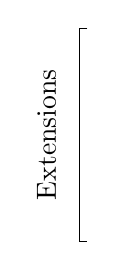
\begin{tikzpicture}\draw (0,0) -- ++(-1mm,0) -- ++(0,-7.7em) node[midway,anchor=base,xshift=-3mm,rotate=90] {Extensions} -- ++(1mm,0);\end{tikzpicture}} &
  \typerule{e=\fix e_1 \qquad \Gamma\vdash e:\T, ~ e_1:\T_1\to\T_2}          % fix
           {\Gamma\vdash e: \T\sqcap\T_2} &
  \typerule{e=e_1/e_2 \qquad \Gamma\vdash e:\T, ~ e_1:\T_1, ~ e_2:\T_2}      % /
           {\renewcommand\arraystretch{1.2}
            \begin{array}[t]{@{}l@{}l@{}}
              \Gamma\vdash{} & e_1:\T_1\sqcap\T, ~ e_2:\T_2\sqcap\T
            \end{array}} & \\
  &
  \typerule{e=[e_1]_{_{cond}} \qquad \Gamma\vdash e:\T,e_1:\T_1}                           % ::
           {\Gamma\vdash e:\T\sqcap\T_1, ~ e_1:\T\sqcap\T_1} &
  \typerule{e=e_1::\T \qquad \Gamma\vdash e:\T_0,e_1:\T_1}                           % ::
           {\Gamma\vdash e:\T\sqcap\T_0\sqcap\T_1, ~ e_1:\T\sqcap\T_0\sqcap\T_1}
\end{array}
\]
\caption{\label{lang:type refinement rules}
  Type refinement rules, for inferring qualifiers in sub-expressions.}
  \vspace{2mm}
\end{figure*}

Base types are inferred normally as in a classical Hindley-Milner type system~\cite{78/Milner}.
The operators (\Cref{lang:operators}) behave like polymorphic
constants with the following types:
\[\renewcommand\arraystretch{1.5}
  \begin{array}{c}
    {\fix} ~:~ \forallT ~(\T\to\T)\to\T \qquad 
    {/} ~:~ \forallT ~\T\to\T\to\T \\
    (::\T) ~:~ \mathrm{shape}[\T]\to\mathrm{shape}[\T]
  \end{array}\]

As for $[\,]_{_\square}$, for all typing purposes the first variant is a no-op, and the second variant
is just syntactic sugar for $:: \square\to\_$\,,
where \,$\_$\, is a fresh type variable.

Any type variables occurring in type expressions are resolved at that
stage through unification. In particular, it means that type variables are always assigned raw types.

Qualifiers are also inferred by propagating them up and down the syntax tree.
Since the program already typechecks once the base types are in place, the problem is no longer
one of finding {\em valid} annotations, but rather of {\em tightening} them as much as possible
without introducing semantics-changing coercions. For example, the term $(f :: I\to(I\cap P))\,i$ may
be assigned the type $I$, but it can also be assigned $I\cap P$ without changing its semantics.

Qualifiers are propagated by defining a \newterm{type intersection} operator $\sqcap$ that
takes two droplets of the same shape $\T_1$, $\T_2$ and returns a droplet with a conjunction of all the qualifiers
occuring in either $\T_1$ or $\T_2$. The operator is defined in terms of the corresponding liquid types:
\begin{itemize}
  \item If $\T_1=\{v:\T ~|~ \varphi_1\}$ and $\T_2=\{v:\T ~|~ \varphi_2\}$,
	\[\T_1\sqcap\T_2 ~=~ \{v:\T ~|~ \varphi_1\land\varphi_2\}\]
  \item If $\T_1=x{\,:\,}\S_1\to\S_2$, $\T_2=x{\,:\,}\S_3\to\S_4$ (normalized so that $\T_1$ and $\T_2$ use the same names for arguments),
    \[\T_1\sqcap\T_2 ~=~ x{\,:\,}(\S_1\sqcap\S_3)\to(\S_2\sqcap\S_4)\]
\end{itemize}

We then define the \newterm{type refinement} steps for terms. They are listed in \Cref{lang:type refinement rules}.
These rules are applied continuously until a fixed point is reached.
The resulting types are eventually converted back to droplet form (expressed via $\cap$ and $\times$);
qualifiers that cannot be expressed in droplets are discarded.

\medskip
The top three rules apply to ordinary constructs of typed $\lambda$-calculus:
the first rule propagates qualifiers from the environment to leaf expressions that use a declared variable;
the next two rules propagate information across application and refinement terms.
For an application $f\,i$, both the type of $i$ and the domain of $f$ can be refined
via the other, e.g. if $f:I_0\to\R$ and $i:I$, then $i$ can be refined to $I_0$; 
symmetrically, if $f:I\to\R$ and $i:I_0$, then $f$ can be refined to $I_0\to\R$.
Similarly, the range of $f$ and the type of $f\,i$ can refine each other.
The rule for abstraction terms is analogous, except that information about the type
of the argument $v$ is passed through the environment.

The bottom rules pertain to language extensions defined previously in this section.
For $/$, qualifiers can safely seep down to sub-expressions (but not back up), e.g. if $x/y:I_0$,
it is safe to assert $x:I_0$, $y:I_0$ without changing the semantics of the expression.
For casts, $x$ and $x::\T$ are tied to have the same refinements, and those
of $\T$ are appended. 
A condition $[x]_{_\square}\,$ ties the sub-term type in the same way, but without
adding any qualifiers. The rule for $\fix$ is the only one that requires some thought:
the type of $\fix f$ cannot be forced down on $f$; but since, by definition, $\fix f = f\,(\fix f)$
must hold, then any restrictions imposed by the range of $f$ can be asserted for $\fix f$.

Note that two syntactically identical terms in different sub-trees may be assigned
different types by this method. This is a desirable property, as (some) context information
gets encoded in the type that way.

The interested reader can find an example of how type inference is applied in \Cref{annex:example:type inference}.

\begin{comment}
\medskip
\examplePar Say $I$, $T$ are types, $\widehat{I}_0 : I\to\B$ a qualifier, $\S$ a type variable, $0:T$ a constant.
The term $(f:I_0\to\S)\,i\mapsto f\,i\,i ~/~ 0$ will induce the following type
inferences:

\begin{tikzpicture}[node distance=1em]
  \node(farg) {$(f:I_0\to\S)$};
  \node(iarg)[right=of farg] {$i$};
  \node(mapsto)[right=of iarg] {$\mapsto$};
  \node(f)[right=of mapsto] {$f$};
  \node(i1)[right=of f] {$i$};
  \node(i2)[right=of i1] {$i$};
  \node(slash)[right=of i2] {$\big/$};
  \node(zero)[right=of slash] {$0$};
  \node(l0)[coordinate,below=1mm of farg] {};
  \node(l1)[coordinate,below=4.5mm of l0] {};
  \node(l2)[coordinate,below=3.5mm of l1] {};
  \node(l3)[coordinate,below=3.5mm of l2] {};
  \node(l4)[coordinate,below=3.5mm of l3] {};
  \def\ytip{2pt}
  \draw (l0 -| farg.west) -- +(0,-\ytip) -| (l0 -| farg.east) node[pos=0.25,below] {\tiny $I_0\to I\to T$};
  \draw (l0 -| iarg.west) -- +(0,-\ytip) -| (l0 -| iarg.east) node[pos=0.25,below] {\tiny $I$};
  \draw (l0 -| f.west) -- +(0,-\ytip) -| (l0 -| f.east) node[pos=0.5,anchor=23,inner xsep=0] {\tiny $I_0\to I\to T$};
  \draw (l0 -| i1.west) -- +(0,-\ytip) -| (l0 -| i1.east) node[pos=0.25,below] {\tiny $I_0$};
  \draw (l0 -| i2.west) -- +(0,-\ytip) -| (l0 -| i2.east) node[pos=0.25,below] {\tiny $I$};
  \draw (l0 -| zero.west) -- +(0,-\ytip) -| (l0 -| zero.east) node[pos=0.25,below] {\tiny $T$};
  \draw (l1 -| f.west) -- +(0,-\ytip) -| (l1 -| i1.east) node[pos=0.25,below] {\tiny $I_0\to T$};
  \draw (l2 -| f.west) -- +(0,-\ytip) -| (l2 -| i2.east) node[pos=0.25,below] {\tiny $T$};
  \draw (l3 -| f.west) -- +(0,-\ytip) -| (l3 -| zero.east) node[pos=0.25,below] {\tiny $T$};
  \draw (l4 -| farg.west) -- +(0,-\ytip) -| (l4 -| zero.east) node[pos=0.25,below] {\tiny $(I_0\to I\to T)\to I\to T$};
\end{tikzpicture}
%\hspace*{\fill}

\noindent
In this case, the type variable $\S$ has been assigned $I\to T$.
\end{comment}

